%!TEX root =  ../main.tex
\renewcommand{\columnseprule}{1.5pt}
\begin{multicols*}{2}
\rule[0.5\baselineskip]{0.4\textwidth}{1pt}
\noindent
\LabSection{Patterns All Around Us}\label{sec:0101p}
\begin{exercises}{sec:0101p}

\lab{} Pick a feature of the room you are in or one nearby.  It should be a repeated, adjacent pattern,
such as carpet squares or ceiling tiles.  In a complete sentence, tell which feature you chose:

\vspace{2cm}
\lab{} Measure the length of one, a few, and several of your items.  There should be some number(s) you
skip over (e.g. 1, 3, 4, and 6).  Record your data below, including units.

\begin{center}%
\begin{tabular}{ c | p{3cm}  }
  \textbf{Number} & \textbf{Length} \\ 
  \hline \hline 
  &  \\ 
  \hline
  &  \\ 
  \hline
  &  \\ 
  \hline
  &  \\ 
  \hline
  &  \\ 
  \hline
\end{tabular}%
\end{center}%
\lab In order to construct a graph, you must
decide on the relationship between the two variables.  Does the number of items depend on
the length, or visa versa?  In other words, decide which one is the \gls{independent variable} and which
is the \gls{dependent variable}.  Justify your choice.

\vspace{2cm}
\lab{} Plot the data points you just observed on a \gls{Cartesian plane}, putting
the independent variable as the left-to-right, and the dependent as the bottom-to-top.
Label your axes and indicate a scale.
Connect your points in a smooth, continuous graph.

\noindent
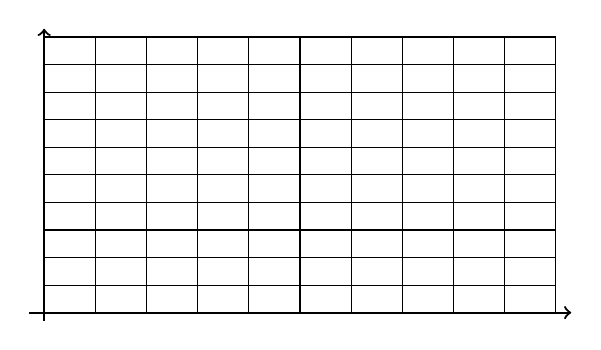
\begin{tikzpicture}[xscale=0.65,yscale=0.35]
	\draw [thick, ->] (-0.3,0) -- (10.3,0);
	\draw [thick, ->] (0,-0.3) -- (0,10.3);
	\draw [thin] (0,0) grid (10,10);
\end{tikzpicture}

\vspace{1cm}

\lab{} Find a \gls{function} that describes your data, and record it in \gls{function notation}.
Call the function $L$ and the argument (i.e. input) $n$.  What kind of function is it?

\vspace{3cm}
\lab{} Not all numbers make sense, either as outputs or inputs to your function.  Conjecture
a reason \gls{domain} and \gls{range} and tell how you arrived at the intervals you did.
Record them below.

\vspace{3cm}
\lab{} When using a \gls{mathematical model}, there are two words to describe going beyond
recorded data:  \gls{interpolation} and \gls{extrapolation}.  
Which prefix means `within' and which means
`without'?  Which word is appropriate to describe finding the missing data point you skipped over from
your observations?  Which would is appropriate to describe finding how long 100 objects 
would be?  Explain your choice.

\vspace{4cm}
\lab{} Describe what you think the point of this problem set is, using technical vocabulary in complete
sentences.
\end{exercises}
\end{multicols*}